\chapter{Benutzeranleitung BananaPi}

\section{Pi Hoch- und Herunterfahren}
Um den Pi Hochzufahren, muss lediglich das Netzteil eingesteckt werden:\\
1. Netzteil in Steckdose einstecken\\
2. Micro-USB Port an den äußeren Port des Pis anschließen. Der andere Port ist nur für OTG!\\
~\\
Um den Pi Herunterzufahren muss benötigt man Zugriff auf die Kommandozeile\\
1. Pi an Tastatur und Bildschirm anschließen || SSH-Verbindung zum Pi aufbauen\\
2. Anmelden (User: root / Passwort: bananapi)\\
3. shutdown -h 0 eingeben und mit ENTER bestätigen\\

\section{Verbindung über SSH}
Um eine Verbindung über SSH aufzubauen wird folgendes benötigt:\\
~\\
- Putty (Windows)\\
- ssh-Packet (Linux)\\
- Netzwerkverbindung\\
~\\
Um eine Verbindung aufzubauen muss der Pi hochgefahren sein und über den Wan-Port an ein Netzwerk angeschlossen sein.
\newpage
\subsection*{Windows:}
1. Putty öffnen\\
2. Hostnamen armbian.bananapihfu.tk angeben
\begin{figure}[ht]
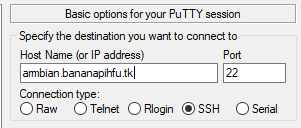
\includegraphics[width=.6\textwidth]{pictures/Jonas/Anleitung/BILD1}
\caption{Eingabe des Hostnamens}
\end{figure}
3. Durch Klick auf „Open“ Verbindung aufbauen -> Terminal öffnet sich
\begin{lstlisting}
login as: root
password: bananapi
\end{lstlisting}
4. Verbindung erfolgreich!

\subsection*{Linux:}
1. Terminal öffnen\\
2. Folgenden Befehl eingeben:
\begin{lstlisting}
ssh root@armbian.bananapihfu.tk
\end{lstlisting}
3. Passwort eingeben:
\begin{lstlisting}
password: bananapi
\end{lstlisting}
4. Verbindung erfolgreich!
\newpage
\section{Lan, Wlan und Vlans}
\subsection*{Übersicht Vlans:}
Der Pi besitzt 4 Lan Ports und einen Wlan Access-Point.\\
~\\
\begin{tabular}{r l}
Vlan 1:   & \\
	- & Internetzugriff\\
	- & Lan 1 + Lan 2\\
	- & Gateway:192.168.1.1\\
Vlan 2:   & \\
	- & Kein Internetzugriff\\
	- & Lan 3 + Lan 4\\
	- & Gateway:192.168.2.1\\
Vlan 3:   & \\
	- & Internetzugriff\\
	- & WLAN AP\\
	- & Gateway:192.168.3.1\\
\end{tabular}

\subsection*{Wlan:}
Der Pi besitzt einen Wlan-AP, über welchen eine Internetverbindung möglich ist. Lokal ist jedoch nur Zugriff auf Geräte im Vlan 3 möglich.
\begin{figure}[ht]

\includegraphics[width=.4\textwidth]{pictures/Jonas/Anleitung/BILD2}
\caption{Die SSID des AP}
\end{figure}
Um eine Verbindung zum AP herzustellen muss folgendermaßen Vorgegangen werden:\\
\begin{tabular}{l l}
1. & Wlan Übersicht am Client Gerät öffnen und nach APs suchen\\
   & a. The BananaPi Project auswählen\\
   & b. WPA/WPA2 PSK auswählen\\
   & c. Passwort: bananapi\\
2. & Verbindung hergestellt\\
\end{tabular}

\subsection*{Lan:}
Der Pi besitzt insgesamt 5 Lan-Ports. Einer davon ist der WAN-Port, welcher an ein externes Netzwerk angeschlossen wird. Die vier restlichen Ports werden über den Pi geroutet und sind in Vlans unterteilt (siehe Übersicht Vlans).

\section{Samba}
\subsection*{Verbindung aufbauen}
Mit Samba können Dateien zwischen dem Pi und einem anderen Gerät ausgetauscht werden.\\
Um den Samba-Share im am eigenen PC einzubinden muss folgendes gemacht werden:\\
~\\
\begin{tabular}{r l}
Windows:& \\
1. & Ausführen-Dialog aufrufen mit Win + R\\
2. & \textbackslash \textbackslash armbian.bananapihfu.tk\textbackslash samba eingeben und mit ENTER bestätigen\\
3. & Login Fenster öffnet sich\\
	& a. Login: sambausr\\
	& b. Passwort: bananapi\\
	& \\
Linux: & \\
1. & smbclient installieren:\\
	& a. sudo apt-get update\\
	& b. sudo apt-get install smbclient\\
2. & Verbindung aufbauen:\\
	& a. smbclient \textbackslash \textbackslash armbian.bananapihfu.tk /samba -U sambausr\\
	& b. Passwort eingeben: bananapi\\
	& \\
MacOSX: & \\
1. & Im Finder mit Server verbinden (Command + K)\\
2. & Serveradresse angeben:\\
	& a. smb://armbian.bananapihfu.tk/samba\\
3. & Verbinden als Registrierter Nutzer:\\
	& a. Name: sambausr\\
	& b. Passwort: bananapi\\
\end{tabular}

\section{Mailserver}
Um auf die Mails zuzugreifen, muss man https://www.google.com/gmail besuchen und sich mit folgenden Benutzerdaten anmelden:\\
- Email: bananapihfu\\
- Passwort: 63!gr\&8FJZdd\\
~\\
Um die Emails über einen Mail-Client aufzurufen, kann die Anleitung von Google zur Hand genommen werden:\\
https://support.google.com/mail/answer/7126229?hl=en

\section{Domainverwaltung}
\subsection*{Ni-IP}
Um die Dynamische DNS bei No-IP zu verwalten muss no-ip.com besucht werden:
- Login: bananapihfu\\
- Passwort: BananaPhone
\begin{figure}[ht]
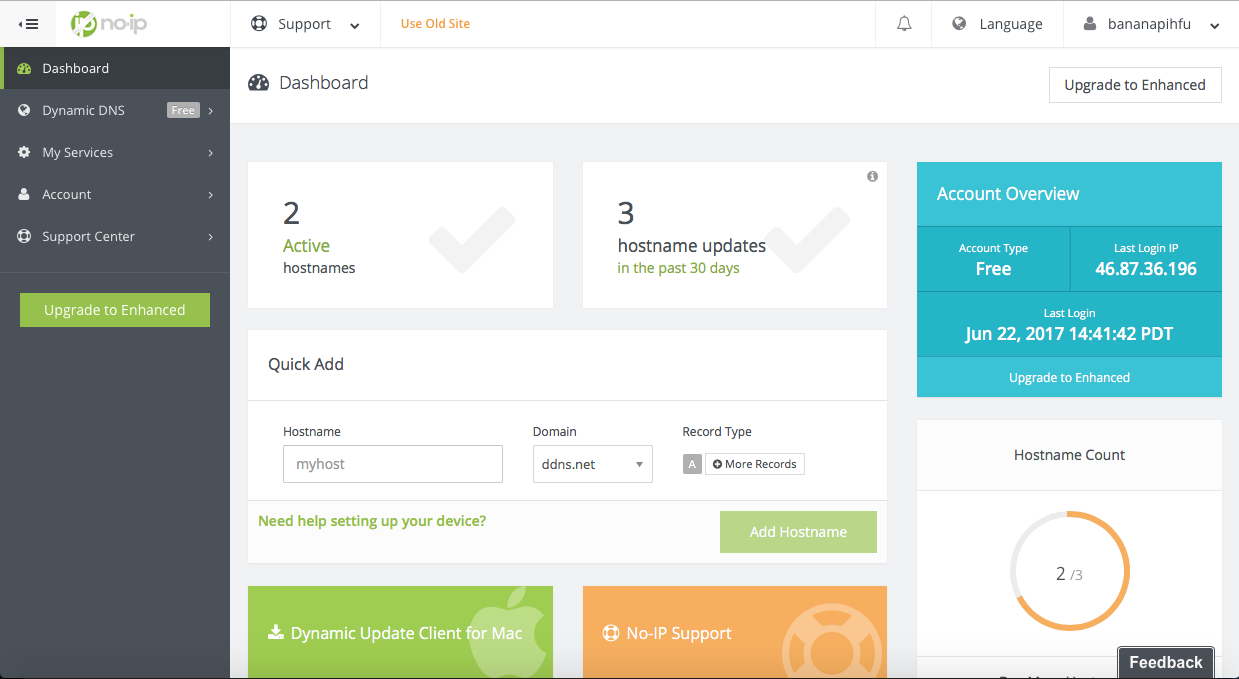
\includegraphics[width=\textwidth]{pictures/Jonas/Anleitung/BILD3}
\caption{No-IP Startseite}
\end{figure}
\newpage
\subsection*{Freenom.com}
Über Freenom wurde die kostenfreie Domain bananapihfu.tk gebucht.\\
Login: bananapihfu@gmail.com\\
Passwort: bananapi
\begin{figure}[ht]
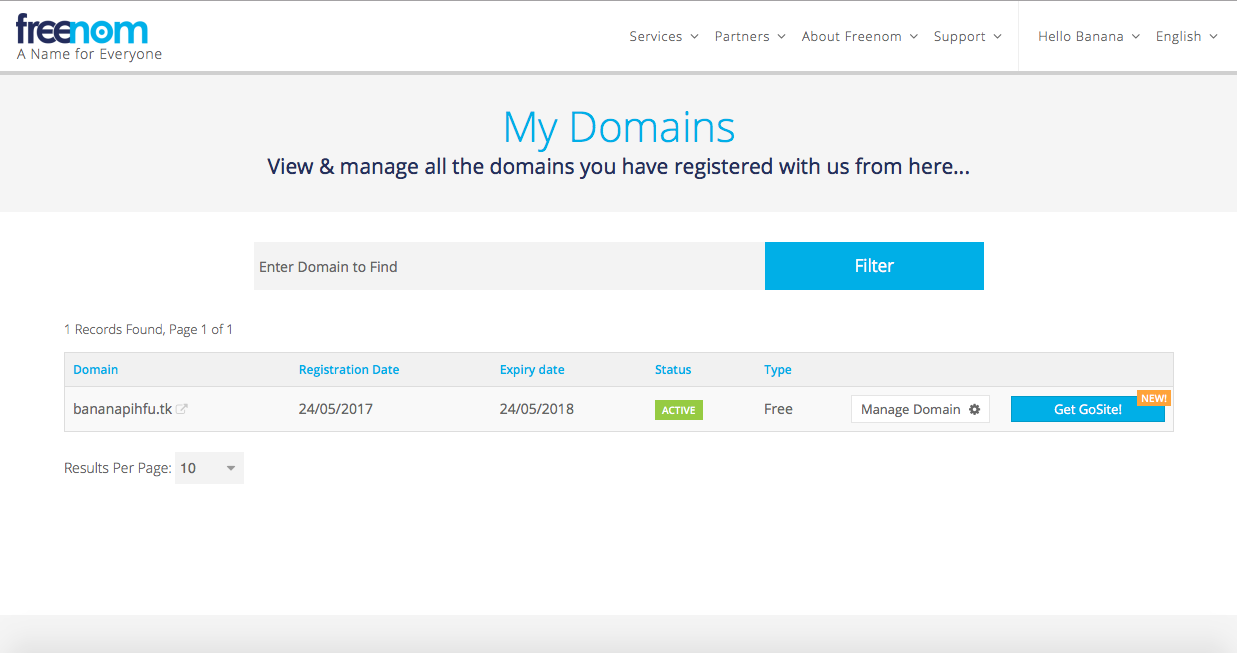
\includegraphics[width=\textwidth]{pictures/Jonas/Anleitung/BILD4}
\caption{Freenom Domainverwaltung}
\end{figure}

\subsection*{CloudFlare}
Über CloudFlare werden die DNS-Einträge der Domain verwaltet:\\
Login: bananapihfu@gmail.com\\
Passwort: k\%KKx!HkNW23
\begin{figure}[ht]
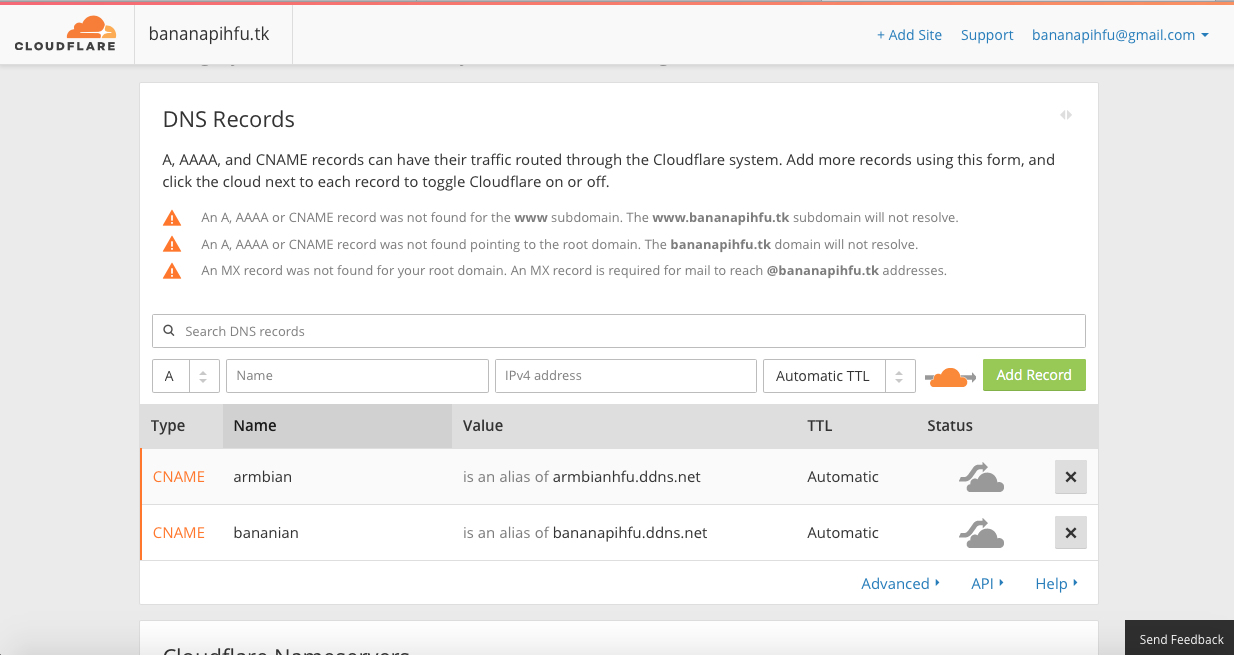
\includegraphics[width=\textwidth]{pictures/Jonas/Anleitung/BILD5}
\caption{Cloudflare DNS}
\end{figure}

\section{Backup und Restore}
Das Backup wird über zwei Skripte gestartet, welche in den Verzeichnissen /etc/cron.weekly/ und /etc/cron.monthly/ liegen. Das Backup wird somit regelmäßig ausgeführt.\\
~\\
Manuelles Backup\\
Sollte man ein aktuelles Backup benötigen, kann man das Backup-Script manuell ausführen:
\begin{lstlisting}
bash /etc/cron.weekly/Backup_Weekly
\end{lstlisting}
Hierbei wird das Backup unter /mnt/SSD/Backup\_Weekly gespeichert.\\
Zur Archivierung des Backups, kann auch das Backup\_Monthly aufgerufen werden:
\begin{lstlisting}
bash /etc/cron.monthly/Backup_Monthly
\end{lstlisting}
Dieses Skript speichert dann das Wöchentliche Backup unter /mnt/SSD/Backup\_Monthly als tar-Archiv.

\section{Statusanzeige}
Die Statusanzeige wird bei Systemstart geöffnet, da das Skript für diese unter /etc/init.d/ abgelegt ist. Das Skript baut eine tmux-Session auf, welche mit folgendem Befehl aufgerufen werden kann:
\begin{lstlisting}
tmux attach 
\end{lstlisting}
Beendet wird die Session mit folgender Tastenkombination:

\begin{lstlisting}
CTRL + D
\end{lstlisting}












